\chapter{Modellierung}
\label{sec:modellierung}
Basierend auf dem Trainingsziel werden die Zyklen mit spezifischer Gewichtung gestaltet. Dabei sind  und Regenerationsphasen Eine Trainingseinheit mit radsportspezifischem Leistungsbereich erfüllt dabei .
Danach fließt in der Phase der konkreten Trainingsplanung die Anforderung und das individuelle Belastungsprofil des Sportlers ein. Regenerationsphasen müssen berücksichtigt werden. 
In der letzten Phase werden die konkreten Trainingseinheiten festgelegt. Diese beinhalten sowohl Trainingsmethoden, als auch Intensität und Dauer der Belastungen. 
Diese Arbeit behandelt ausschließlich die initiale Erstellung eines Trainingsplans. Es erfolgt keine Trainingssteuerung durch Dokumentation oder Kontrolle.

    
Die Anforderungen aus der Trainingswissenschaft bilden als mathematisches Modell die Grundlage für den Algorithmus. 
% Profi (Trainingsumfang > 20h)

% Amateur (Trainingsumfang < 20h)

% Hobbyfahrer (Trainingsumfang < 4h)

\section{Übersicht}
\label{sec:modellierung:uebersicht}
    \begin{enumerate}
        \item Trainingsziel bestimmen
        \item Einfach-Periodisierung des Trainingplans zum Wettkampfstermin
        \item Vierfach-Periodisierung der Aufbauphase aus Vorbereitungsperioden
        \item Constraints auf jeder Ebene der Hierarchie definieren 
        \item Solver erstellt Trainingseinheiten
    \end{enumerate}
    \subsection{hierarchische Zyklisierung}
    \begin{figure}[htb]
    	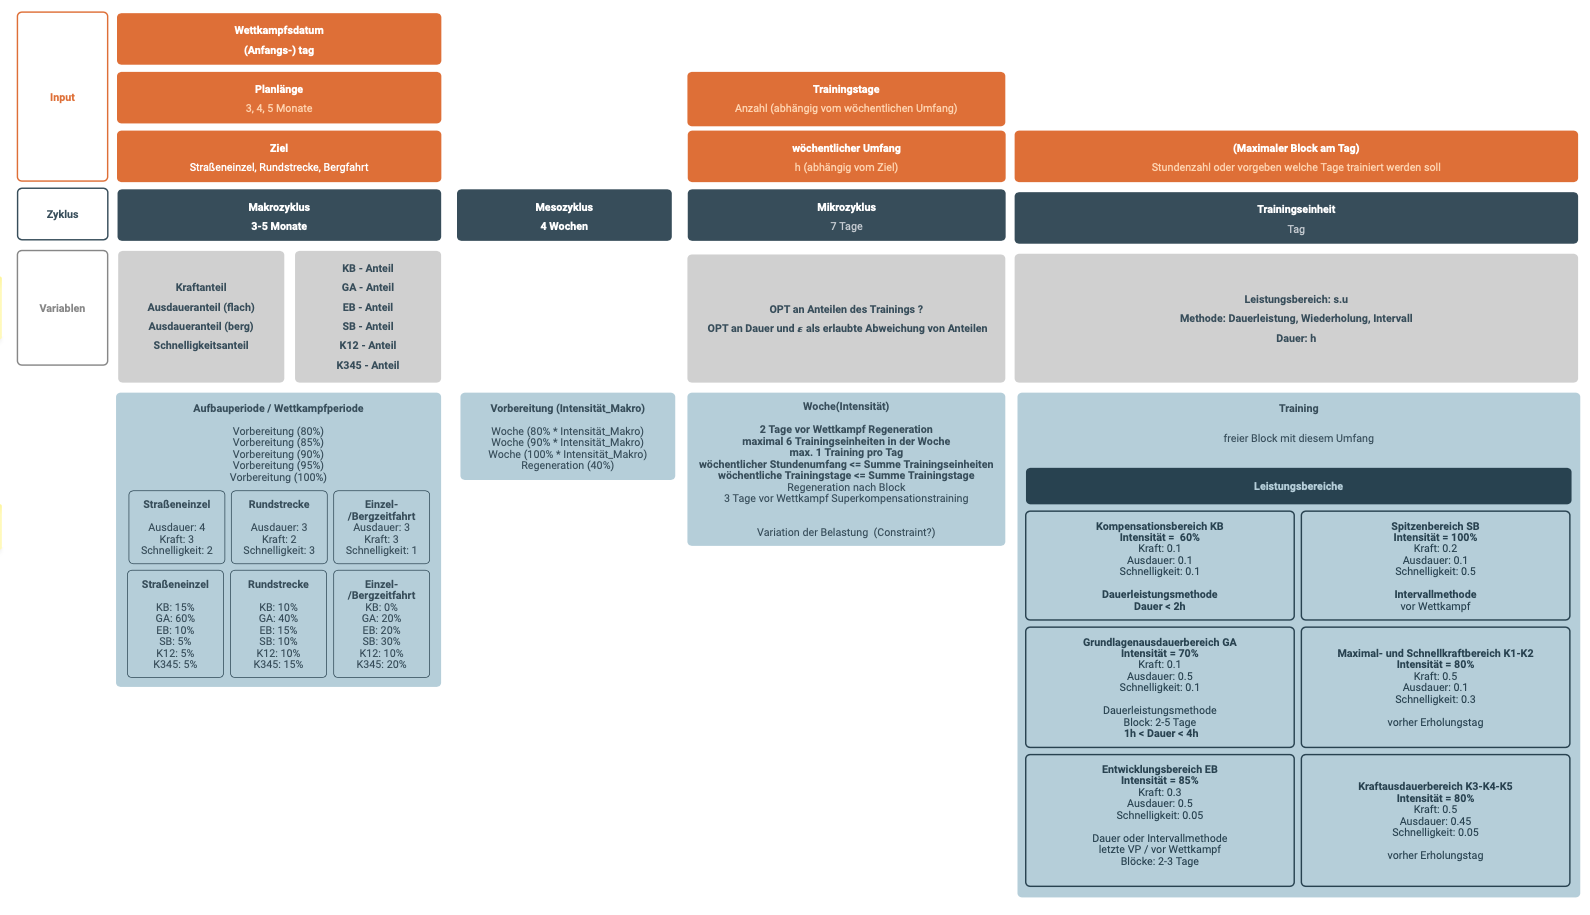
\includegraphics[width=\textwidth]{gfx/modell.png}
    	\caption{Schema aus Makro-, Meso- und Mikrozyklen}
    	\label{fig:modellierung:schema}
    \end{figure}


\section{Benutzer}
\subsection{Input}
\begin{itemize}
    \item maximaler wöchentlicher Trainingsumfang: Anzahl Stunden
    \item maximale wöchentliche Trainingstage: Anzahl Tage
    \item Wettkampfstermin: Datum
    \item Dauer des Plans: 3/4/5 Monate
    \item Ziel/Disziplin \cite[S.11]{Radsporttraining} unterschiedlicher Gewichtung\cite[S.14]{Radsporttraining}
    \begin{itemize}
        \item Straßeneinzelrennen
        \item Rundstrecke
        \item Bergzeitfahrt
    \end{itemize}
    \item ? maximale Stunden für jeden Wochentag: h/Tag
\end{itemize}
\subsection{Output}
Liste von Trainingseinheiten
\label{sec:modellierung:output}
    \begin{itemize}
        \item Tag: Datum
        \item Dauer: Anzahl h
        \item Trainingsbereich: \ref{tab:trainingsbereiche}
        \item Trainingsmethode: $\{Dauerleistung, Intervall, Wiederholung\}$
        \item ? Trainingsalternativen = Auswahl an möglichen Einheiten
    \end{itemize}
    
\section{Model}
    \subsection{Variablen}
        Input maximaler wöchentlicher Trainingsumfang (Stunden)
        $max_{hours} \in [0, 40]$
        
        Input maximale Anzahl der Trainingstage in einer Woche
        $max_{days} \in [1, 7]$
        
        Input Trainingsziel
        \TODO{Anteile Leistungsbereiche oder K/A/S}
        $strength \in [0, 100]$
        $endurance \in [0, 100]$        
        $speed \in [0, 100]$
                
        Input Wettkampfstag -> Trainingslänge = Anzahl der Tage
        $length \in \{ 84, 112, 140\} $ 
        
        Variable um den Tag der Trainingseinheit $i$ zu identifizieren
        \begin{equation}
            \forall i \in [1, \text{length}], \text{day}_i = [\![1, \text{length}]\!]
        \end{equation}
    
        Variable um Leistungsbereich der Trainingseinheit $i$ zu identifizieren
        \begin{equation}
            \forall i \in [1, \text{length}], \text{range}_i = [\![0, 6]\!] \text{oder} \{\text{KB, GA, EB, SB, K12, K345}\}
        \end{equation}
        
        Variable um Dauer der Trainingseinheit $i$ zu identifizieren
        \begin{equation}
            \forall i \in [1, \text{length}], \text{duration}_i = [\![0, 10]\!]
        \end{equation}
        
        Variable um Trainingsmethode der Trainingseinheit i zu identifizieren
        \begin{equation}
            \forall i \in [1, \text{length}], \text{method}_i = \{\text{DL, IV, WH}\}
        \end{equation}

    \subsection{Constraints}
    \subsubsection{Allgemein}
    Nur ein Training pro Tag
        \begin{equation}
            \forall i, j \in [1, 150]^2, i\neq j \Rightarrow day_i \neq day_j
        \end{equation}
    Summe der Trainingsstunden unter wöchentlichem Umfang
    \TODO{Definition einer einzelnen Woche}
        \begin{equation}
            \forall i = k * 7 + 1, k \in \math{Z}, \sum_{i}^{i+6} \text{duration}_i \leq max_{hours}
        \end{equation}
        \begin{equation}
            \forall i \in \{ i = k * 7 + 1, k \in \math{Z} \}, \sum_{i}^{i+6} \text{duration}_i \leq max_{hours}
        \end{equation}
    Summe der Trainingstage unter wöchentlichem Maximalwert
        \begin{equation}
            \forall i = k * 7 + 1, k \in \math{Z}, \sum_{i}^{i+6} \text{day}_i \leq max_{days}
        \end{equation}
    Maximal 6 Trainingseinheiten in der Woche
        \begin{equation}
            max_{days} \leq 6
        \end{equation}
    3 Tage vor Wettkampf kein Training (Superkompensation)
    \TODO{duration = 0 oder kein Training?}
        \begin{equation}
            \forall i \in [\text{length}-3, \text{length}] \in \math{Z}, \sum_{i}^{i+6} \text{day}_i \leq max_{days}
        \end{equation}

    \subsubsection{Trainingseinheit}
    KB Einheit hat maximale Dauer von zwei Stunden
        \begin{equation}
            \forall i \in \{i | \text{range}_i = \text{KB}\}, \text{duration}_i \leq 2
        \end{equation}
    KB Einheit immer als Dauerleistungsmethode
        \begin{equation}
            \forall i \in \{i | \text{range}_i = \text{KB}\}, \text{method}_i = \text{DL}
        \end{equation}
    GA Einheit hat Mindestdauer von 1 Stunde
        \begin{equation}
            \forall i \in \{i | \text{range}_i = \text{GA}\}, 1 \leq \text{duration}_i
        \end{equation}
    GA Einheit hat maximale Dauer von fünf Stunden
        \begin{equation}
            \forall i \in \{i | \text{range}_i = \text{GA}\}, \text{duration}_i \leq 5
        \end{equation}
    GA Einheit immer als Dauerleistungsmethode
        \begin{equation}
            \forall i \in \{i | \text{range}_i = \text{GA}\}, \text{method}_i = \text{DL}
        \end{equation}
    SB Einheit immer als Intervallmethode
        \begin{equation}
            \forall i \in \{i | \text{range}_i = \text{SB}\}, \text{method}_i = \text{IV}
        \end{equation}
        
    \subsubsection{Optimierung}
    OPT an Anteilen des Trainings 
        \begin{equation}
            \forall i \in \{i | \text{range}_i = \text{KB}\}, \text{method}_i = \text{DL}
        \end{equation}
    Alternative: OPT an Dauer \TODO{mit erlaubter Abweichung $\epsilon$ der Gewichtungen}
        \begin{equation}
            \text{minimize: } \sum_{i=0}^{\text{length}} \text{duration}_i
        \end{equation}
    
    
    \subsubsection{Notizen}
        \begin{itemize}
            \item nur x aufeinanderfolgende Tage
            \item GA Trainings am Besten als Block \cite[34]{Radsporttraining}ku
        \end{itemize}
\section{Solver}
    